
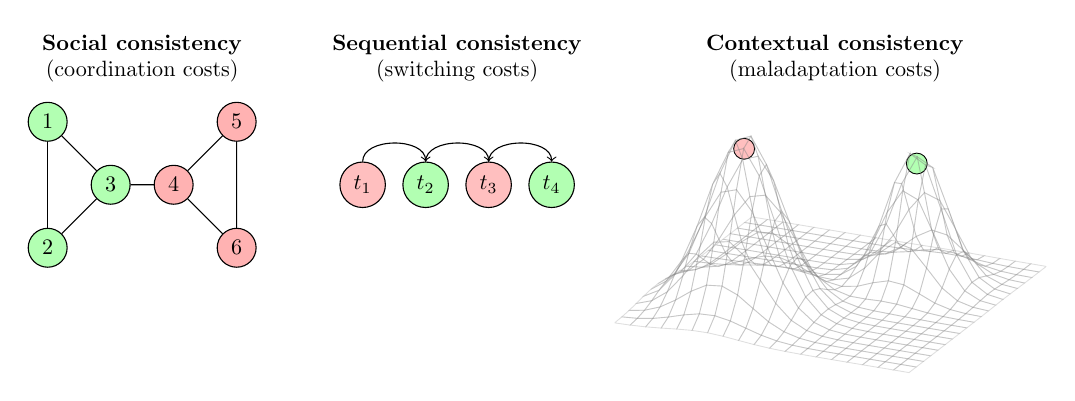
\begin{tikzpicture}[scale=0.8, transform shape]

% \draw [decorate,decoration={brace,amplitude=5pt,raise=4ex}]
%   (-1,1) -- (-1,6) node[midway,rotate=90,yshift=+4em,align=center]{\textbf{Convention}\\\textbf{optimality}};

\begin{scope}[shift={(0,3)}]
    \node[circle, draw, fill=red!30] (D) at (2,2) {5};
    \node[circle, draw, fill=red!30] (E) at (2,0) {6};
    \node[circle, draw, fill=red!30] (F) at (1,1) {4};

    % Left graph (traditional)
    \node[circle, draw, fill=green!30] (A) at (-1,2) {1};
    \node[circle, draw, fill=green!30] (B) at (-1,0) {2};
    \node[circle, draw, fill=green!30] (C) at (0,1) {3};


    \draw (A) -- (B);
    \draw (B) -- (C);
    \draw (C) -- (A);
    \draw (D) -- (E);
    \draw (E) -- (F);
    \draw (F) -- (D);

    \draw (F) -- (C);

    \node[align=center] (label) at (0.5,3) {\textbf{Social consistency}\\(coordination costs)};
\end{scope}

\begin{scope}[shift={(4,4)}]
    \node[draw,circle,fill=pink] (a) at (0,0) {$t_1$};
    \node[draw,circle,fill=green!30] (b) at (1,0) {$t_2$};
    \node[draw,circle,fill=pink] (c) at (2,0) {$t_3$};
    \node[draw,circle,fill=green!30] (d) at (3,0) {$t_4$};
    \draw[->,bend right=90] (a.north) to [out=90,in=90] (b.north);
    \draw[->,bend right=90] (b.north) to [out=90,in=90] (c.north);
    \draw[->,bend right=90] (c.north) to [out=90,in=90] (d.north);

    \node[align=center] (label) at (1.5,2) {\textbf{Sequential consistency}\\(switching costs)};
\end{scope}

\begin{scope}[shift={(8,0)}]
\begin{scope}[shift={(0,0.75)}]
\begin{axis}[hide axis]
\node[draw,circle,fill=pink] at (axis cs:-1, -1, +1.05) {};
\node[draw,circle,fill=green!30] at (axis cs:1, 1, +0.80) {};
\addplot3 [
domain=-2.5:2.5,
domain y = -2.5:2.5,
samples = 20,
samples y = 20,
surf,
opacity=0.25,
fill=white,
fill opacity=0.01,
faceted color = gray] {+1.15*exp(-((x+1)^2+(y+1)^2)/0.67)+0.9*exp(-((x-1)^2+(y-1)^2)/0.4)};
\end{axis}
\end{scope}

\node[align=center] (label) at (3.5,6) {\textbf{Contextual consistency}\\(maladaptation costs)};
\end{scope}

\end{tikzpicture}